%%%%%%%%%%%%%%%%%%%%%%%%%%%%%%%%%%%%%%%%%
% Beamer Presentation
% LaTeX Template
% Version 1.0 (10/11/12)
%
% This template has been downloaded from:
% http://www.LaTeXTemplates.com
%
% License:
% CC BY-NC-SA 3.0 (http://creativecommons.org/licenses/by-nc-sa/3.0/)
%
%%%%%%%%%%%%%%%%%%%%%%%%%%%%%%%%%%%%%%%%%

%----------------------------------------------------------------------------------------
%	PACKAGES AND THEMES
%----------------------------------------------------------------------------------------

\documentclass[compress]{beamer}

\mode<presentation> {

% The Beamer class comes with a number of default slide themes
% which change the colors and layouts of slides. Below this is a list
% of all the themes, uncomment each in turn to see what they look like.

%\usetheme{default}
%\usetheme{AnnArbor}
%\usetheme{Antibes}
%\usetheme{Bergen}
%\usetheme{Berkeley}
\usetheme{Berlin}
%\usetheme{Boadilla}
%\usetheme{CambridgeUS}
%\usetheme{Copenhagen}
%\usetheme{Darmstadt}
%\usetheme{Dresden}
%\usetheme{Frankfurt}
%\usetheme{Goettingen}
%\usetheme{Hannover}
%\usetheme{Ilmenau}
%\usetheme{JuanLesPins}
%\usetheme{Luebeck}
%\usetheme{Madrid}
%\usetheme{Malmoe}
%\usetheme{Marburg}
%\usetheme{Montpellier}
%\usetheme{PaloAlto}
%\usetheme{Pittsburgh}
%\usetheme{Rochester}
%\usetheme{Singapore}
%\usetheme{Szeged}
%\usetheme{Warsaw}

% As well as themes, the Beamer class has a number of color themes
% for any slide theme. Uncomment each of these in turn to see how it
% changes the colors of your current slide theme.

%\usecolortheme{albatross}
%\usecolortheme{beaver}
%\usecolortheme{beetle}
%\usecolortheme{crane}
%\usecolortheme{dolphin}
%\usecolortheme{dove}
%\usecolortheme{fly}
%\usecolortheme{lily}
%\usecolortheme{orchid}
%\usecolortheme{rose}
%\usecolortheme{seagull}
%\usecolortheme{seahorse}
%\usecolortheme{whale}
%\usecolortheme{wolverine}

%\setbeamertemplate{footline} % To remove the footer line in all slides uncomment this line
\setbeamertemplate{footline}[page number] % To replace the footer line in all slides with a simple slide count uncomment this line

%\setbeamertemplate{navigation symbols}{} % To remove the navigation symbols from the bottom of all slides uncomment this line
}

\usepackage{graphicx} % Allows including images
\usepackage{booktabs} % Allows the use of \toprule, \midrule and \bottomrule in tables
\usepackage{color}
\usepackage{mathrsfs}
\usepackage{type1cm}
\newcommand{\ty}{\fontsize{4pt}{6pt}\selectfont}
\setbeamertemplate{caption}[numbered]

% image directory
\graphicspath{{imgs/}}

% font
\usepackage{times}
\usefonttheme{professionalfonts}

% caption font size
\usepackage{caption}
\captionsetup{font={small}}

\usepackage{comment}
\usepackage{multirow}

% pseudo-code
\usepackage{algorithm}
\usepackage[noend]{algpseudocode}


\hypersetup{
  pdfauthor={Liu Weizhi},
  pdfpagemode=FullScreen,
  colorlinks={true}
}
%----------------------------------------------------------------------------------------
%	TITLE PAGE
%----------------------------------------------------------------------------------------

\title[IE5504 Project]{Solving Multi-armed Bandit Problems \\ Based on Simulation Optimization} % The short title appears at the bottom of every slide, the full title is only on the title page

\author{Li Qingxuan, Liu Weizhi, Yuan Yuhe, Wong Manyu} % Your name
\institute[NUS ISE] % Your institution as it will appear on the bottom of every slide, may be shorthand to save space
{
Department of Industrial \& Systems Engineering \\ National University of Singapore \\ % Your institution for the title page
\medskip
%\textit{weizhiliu2009@gmail.com} % Your email address
}
\date{\today} % Date, can be changed to a custom date

\begin{document}
\small

\begin{frame}
\titlepage % Print the title page as the first slide
\end{frame}

\begin{frame}
\frametitle{Overview} % Table of contents slide, comment this block out to remove it
\tableofcontents % Throughout your presentation, if you choose to use \section{} and \subsection{} commands, these will automatically be printed on this slide as an overview of your presentation
\end{frame}

%----------------------------------------------------------------------------------------
%	PRESENTATION SLIDES
%----------------------------------------------------------------------------------------

\section{Introduction}
\subsection{}
\begin{frame}
\frametitle{Multi-armed Bandit}
\begin{itemize}
  \item Origin: How to play slot machines wisely in casino?
       \begin{columns}
       \column{.5\textwidth}
        \begin{figure}[htb!]
          \centering
          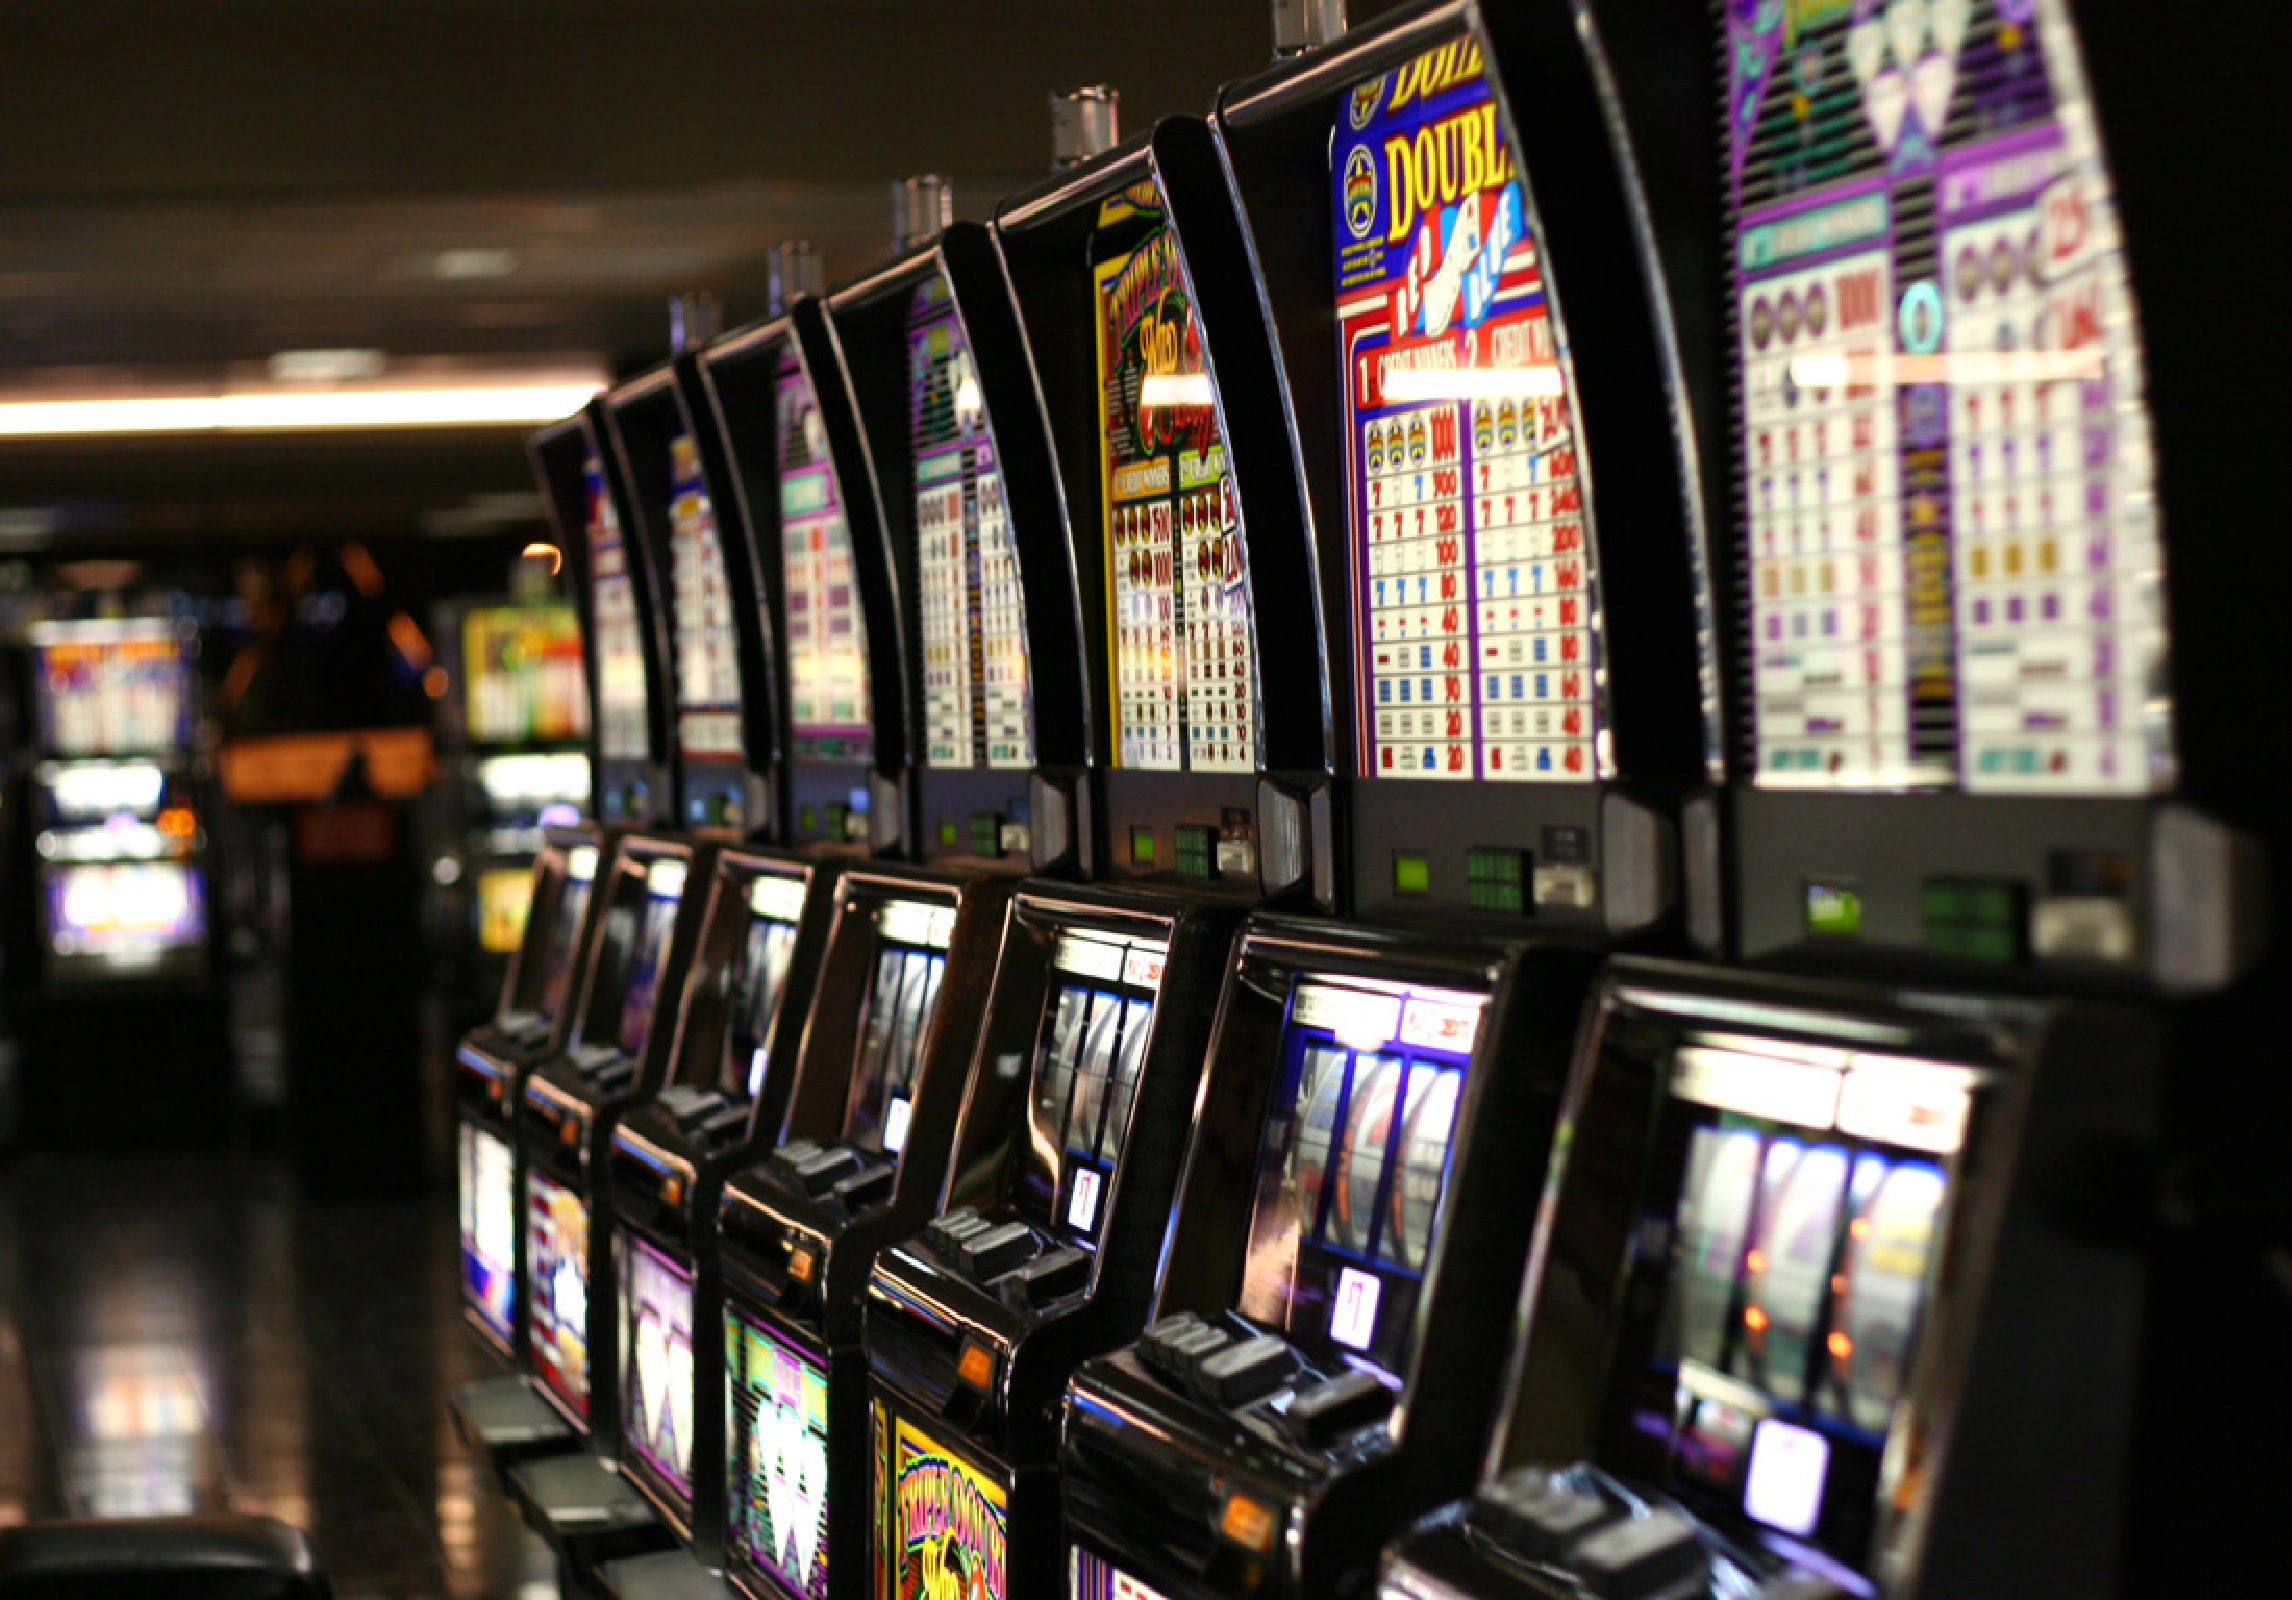
\includegraphics[width=0.6\textwidth]{casino.pdf}
          \caption{\label{fig:casino} Slot Machines in Casino}
        \end{figure}
       \column{.5\textwidth}
        \begin{figure}[htb!]
          \centering
          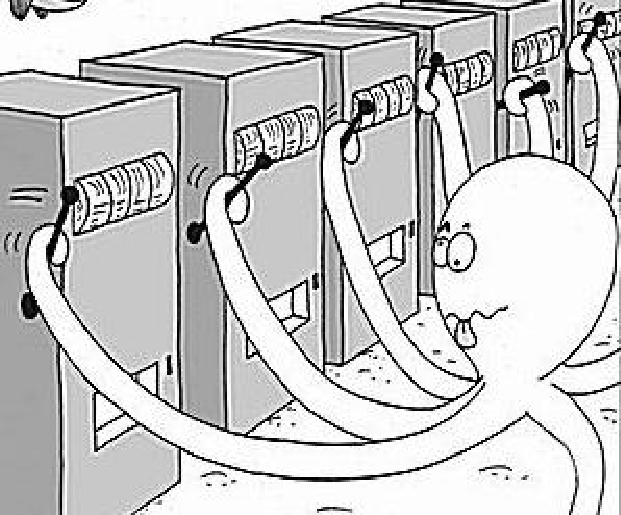
\includegraphics[width=0.5\textwidth]{mab.pdf}
          \caption{\label{fig:mab} Multi-armed Bandit}
        \end{figure}       
      \end{columns}
  \item \textbf{Task: Maximize your total reward $R$ with at most $N$ trials given $K$ slot machines to play, whose reward distribution is different.}
  \item Application: online advertising (A/B testing), clinical trials, adaptive routing, dynamic allocation, etc.
\end{itemize}
\end{frame}

\begin{frame}
\frametitle{Problem Formulation}
\begin{itemize}
  \item Assumption: To simplify the problem without loss of generality, we assume \textbf{the reward of slot machine (also called Arm) $i$ follows Bernoulli distribution with success rate $p_{i}, i = 0,1,\cdots,K-1$. }
  \item Challenges:
    \begin{itemize}
      \item Exploration vs. Exploitation Dilemma \\
           \textit{``Bandit problems embody in essential form a conflict evident in all human action: choosing actions which yield immediate reward ({\color{red}exploit current best}) vs. choosing actions whose benefit will come only later ({\color{red}explore unknown solution}).''  (P.Whittle 1980)}
      \item Value of history information \\
            {\color{red}How to analyze history reward to evaluate each arm?}
      \item Confidence of optimal arm \\
            {\color{red}How confident do you believe the estimated optimal arm is the true optimal?}
    \end{itemize}
\end{itemize}
\end{frame}

\section{Methods}

\subsection{}

\begin{frame}
\frametitle{Notations}
\begin{table}[htbp]
  \tiny
  \centering
  \caption{Notations}
    \begin{tabular}{ccc}
    \toprule
    Notation &  Definition & Remarks\\
    \midrule
    $p_{i}$ & true success rate for Arm $i$ & $p_{i} \in [0,1]$\\    
    ${\color{red}\Tilde X_{i}}$ & average reward of Arm $i$ & $\Tilde X_{i} \sim N(\mu_{i}, \frac{\sigma_{i}^{2}}{N_{i}})$ \\
    {\color{red}$\vec r_{i}$} & current reward history for Arm $i$ & $\vec r_{i} = [X_{i1}, X_{i2}, \cdots, X_{i t_{i}}]$ \\
    {\color{red}$R_{i}$} & current total reward for Arm $i$ & $R_{i} = \vec r_{i} e^{T}$ \\
    {\color{red}$N_{i}$} & current total number of draw for Arm $i$ & the length of $\vec r_{i}$ \\
    {\color{red}$\hat N_{i}$} & estimated next total number of draw for Arm $i$ & please refer to OCBA \\
    $\mu_{i}$ & sample mean of $\vec r_{i}$ & $\mu_{i} = \frac{1}{N_{i}} R_{i}$ \\
    $\sigma_{i}^{2}$ & sample variance of $\vec r_{i}$ & $\sigma_{i}^{2} = \frac{1}{N_{i} - 1} \sum_{k=1}^{t_{i}} (X_{ik} - \mu_{i})^{2}$ \\
    {\color{red}$\Tilde p_{i}$} & sample point of success rates & $\Tilde p_{i} \sim \mbox{Beta}(R_{i}+1, N_{i}-R_{i}+1)$ \\
    $\tau$ & exploration weight for ucb value & please refer to UCB \\
    \bottomrule
    \end{tabular}%
  \label{tab:notations}%
\end{table}%
\end{frame}

\subsection{Method 1 - Upper Confidence Bounds Algorithm}

\begin{frame}
\frametitle{Exploration/Exploitation Dilemma - UCB}
\begin{itemize}
  \item Main Idea: Automatic balance exploration/exploitation dilemma based on ucb value. 
  \item Procedure:
    \begin{itemize}
      \item Step 1: Draw each Arm $i (i = 0, 1, \cdots, K-1)$ once and update $\vec r_{i}$ and $N_{i}$.
      \item Step 2: Update ucb value for each Arm $i$
                    \begin{align}
                      ucb_{i} & = \frac{R_{i}}{N_{i}} + \tau \sqrt{\frac{2 \log \sum_{i=0}^{K-1} N_{i}}{N_{i}}}
                    \end{align}
      \item Step 3: Select Arm $b = \arg \max_{i} ucb_{i}$ to draw, and update $\vec r_{b}$ and $N_{b}$.
      \item Step 4: Return to Step 2 until total budget run out.
    \end{itemize}
\end{itemize}
\end{frame}

\subsection{Method 2 - Bayes Bandit Algorithm}

\begin{frame}
\frametitle{History Information - Bayes Bandit}
\begin{itemize}
  \item Main Idea:
    \begin{itemize}
      \item Generate posterior distribution $f(\theta | x)$ given prior distribution $f(\theta)$ and history information $x$
            \begin{align}
              f(\theta | x) & = \frac{f(x | \theta) f(\theta)}{\int_{Y} f(y | \theta) f(\theta) dy }
            \end{align}
      \item In our problem, we have to estimate the distribution of success rate $\Tilde p_{i}$ for each arm.            
      \item The conjugate prior distribution of likelihood function $f(x | \theta)$ could guarantee the same formulation between prior and posterior distribution.
      \item Binomial likelihood function has conjugate prior distriubtion $\mbox{Beta}(\alpha + 1, \beta + 1)$, where $\alpha, \beta$ are the success and failure times.
      \item $\mbox{Beta}(1,1)$ is just the $\mbox{Uniform}(0,1)$
    \end{itemize}
\end{itemize}
\end{frame}

\begin{frame}
\frametitle{History Information - Bayes Bandit}
\begin{itemize}
  \item Procedure:
    \begin{itemize}
      \item Step 1: Sample success rates $\Tilde p_{0}, \cdots, \Tilde p_{K-1}$ for each arm from its prior distribution $\mbox{Beta}(R_{i} + 1, N_{i} - R_{i} + 1)$.
      \item Step 2: Select Arm $b = \arg \max_{i} \Tilde p_{i}$ to draw, and update $\vec r_{b}$ and $N_{b}$.
      \item Step 3: Return to Step 1 until total budget run out.
    \end{itemize}
\end{itemize}
\end{frame}

\subsection{Method 3 - Optimal Computing Budget Allocation}

\begin{frame}
\frametitle{Confidence of Optimal Arm - OCBA}
\begin{itemize}
  \item Main Idea: Maximize the probability of correct selection based on wise allocation rules.
                  \begin{scriptsize}
                  \begin{align}
                    APCS & = 1 - \sum_{i=0, i \neq b}^{K-1} P \{\Tilde X_{b} < \Tilde X_{i} \} & = 1 - \sum_{i=0, i \neq b}^{K-1} \Phi(\frac{\mu_{i} - \mu_{b}}{\sqrt{\frac{\sigma_{b}^{2}}{N_{b}} + \frac{\sigma_{i}^{2}}{N_{i}}}})
                  \end{align}
                  \end{scriptsize}
\end{itemize}
\end{frame}

\begin{frame}
\frametitle{Confidence of Optimal Arm - OCBA}
\begin{itemize}
  \item Procedure:
    \begin{itemize}
      \item Step 1: Draw each Arm $i$ for $n_{0}$ times and update $\vec r_{i}$ and $N_{i}$.
      \item Step 2: Calculate the sample mean $\mu_{i}$ and sample variance $\sigma_{i}^{2}$ based on $\vec r_{i}$ for each Arm $i$. Then find current best Arm $b = \arg \max_{i} \mu_{i}$.
      \item Step 3: Increase the computing budget by 1 and compute the next allocation rule
                    \begin{scriptsize}
                    \begin{align}
                      \frac{\hat N_{i}}{\hat N_{j}} = (\frac{\sigma_{i} (\mu_{b} - \mu_{j})}{\sigma_{j} (\mu_{b} - \mu_{i})})^{2}, i \neq j \neq b & \quad \hat N_{b} = \sigma_{b} \sqrt{\sum_{i=0,i \neq b}^{K-1} (\frac{\hat N_{i}}{\sigma_{i}})^{2} } \\
                      \sum_{i=0}^{K-1} \hat N_{i} & = \sum_{i=0}^{K-1} N_{i} + 1
                    \end{align}
                    \end{scriptsize}
       \item Step 4: Select Arm $k = \arg \max_{i} (\hat N_{i} - N_{i})$ to draw and update $\vec r_{k}$ and $N_{k}$.
       \item Step 5: Return to Step 2 until total budget run out.
    \end{itemize}
\end{itemize}
\end{frame}



\section{Results and Analysis}

\subsection{}

\begin{frame}
Main Experiments
\begin{itemize}
\item Change of the Best Arm Winning Probability
\item Change in Budget
\item Change in Initial Budget (OCBA)
\item Comparison of Efficiency
\end{itemize}
\end{frame}

\subsection{Change of the Best Arm Winning Probability}

\begin{frame}
\begin{figure}[p]
    \centering
    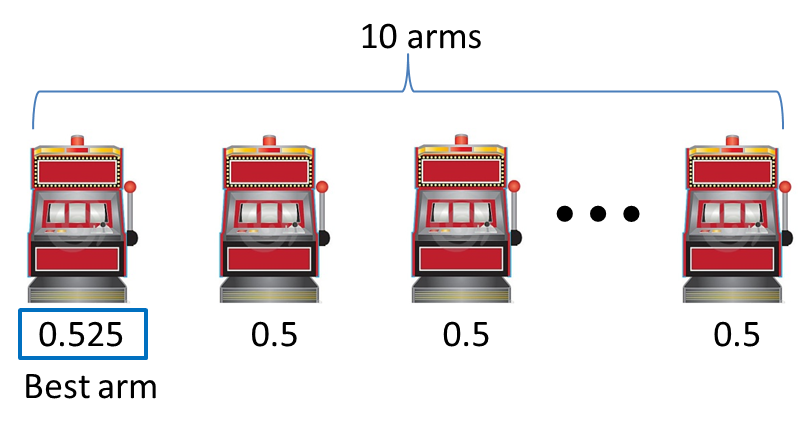
\includegraphics[width=0.8\textwidth]{arms.png}
\end{figure}
\begin{itemize}
\item Variation of the Best Arm Winning Probability while keeping the Winning Probability of all other arms at 0.5
\end{itemize}
\end{frame}

\begin{frame}
\smaller
\begin{minipage}{0.48\textwidth}
\begin{figure}[p]
    \centering
    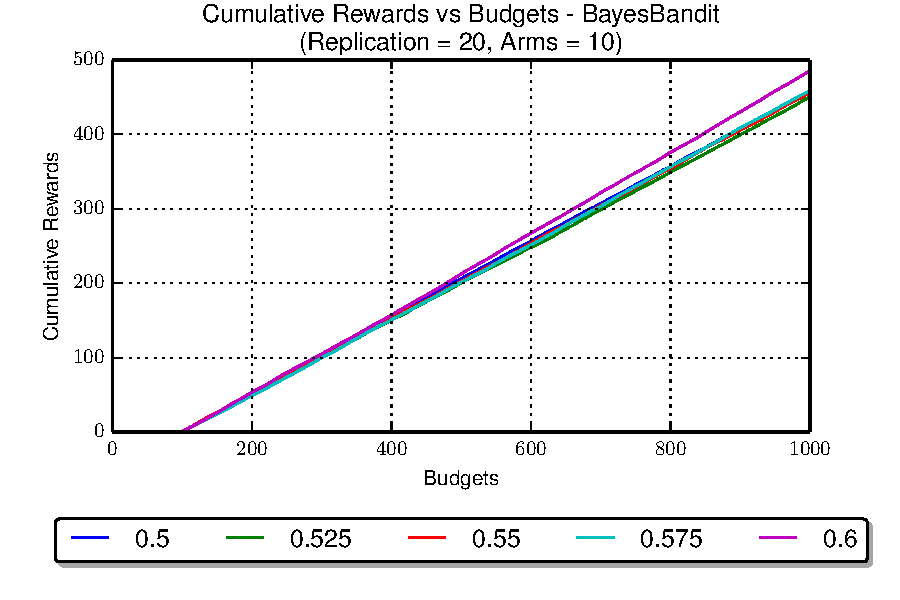
\includegraphics[page=1,width=\textwidth]{1BayesBandit_rate_series_cumulative_rewards.pdf}
\end{figure}
\begin{figure}[p]
    \centering
    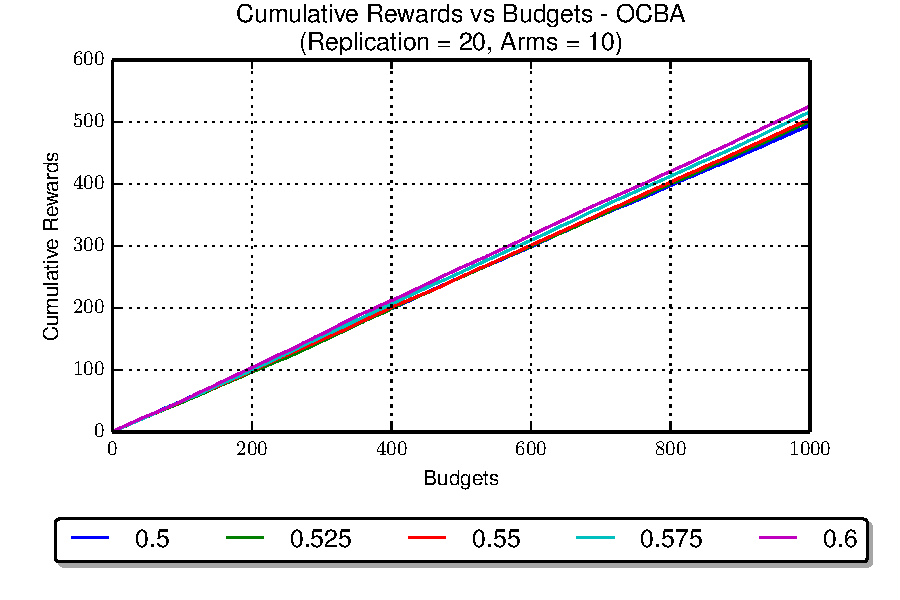
\includegraphics[page=1,width=\textwidth]{2OCBA_rate_series_cumulative_rewards.pdf}
\end{figure}
\end{minipage}%
\hfill
\begin{minipage}{0.48\textwidth}
\begin{tabular}{p{\textwidth}}
\begin{figure}[p]
    \centering
    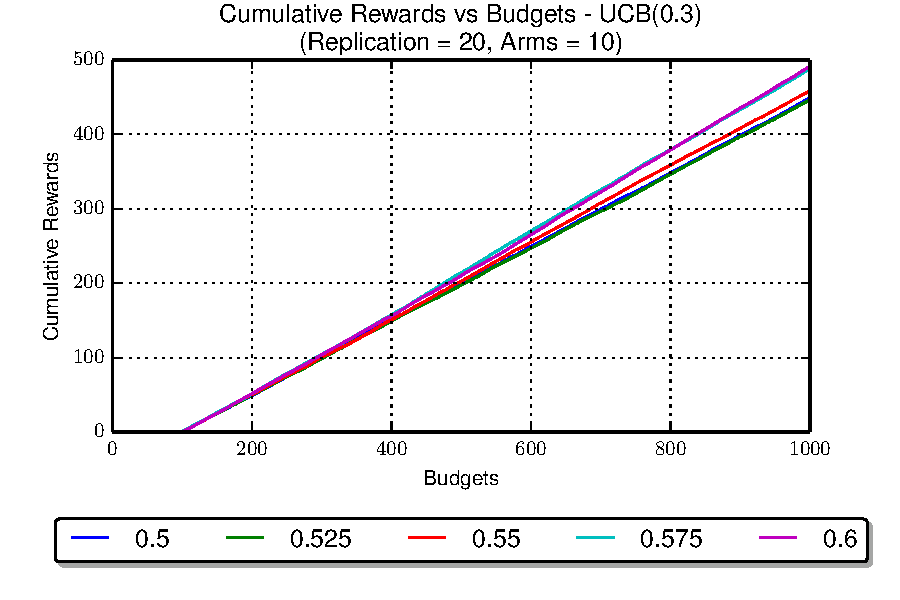
\includegraphics[page=1,width=\textwidth]{3UCB_rate_series_cumulative_rewards.pdf}
\end{figure}
\begin{itemize}
\item Difference in cumulative reward increases as time goes on. \\
\item Least obvious in OCBA.\\
\item Most obvious in the UCB case. (Small Critical Difference)
\end{itemize}
\end{tabular}
\end{minipage}%
\end{frame}

\begin{frame}
\smaller
\begin{minipage}{0.48\textwidth}
\begin{figure}[p]
    \centering
    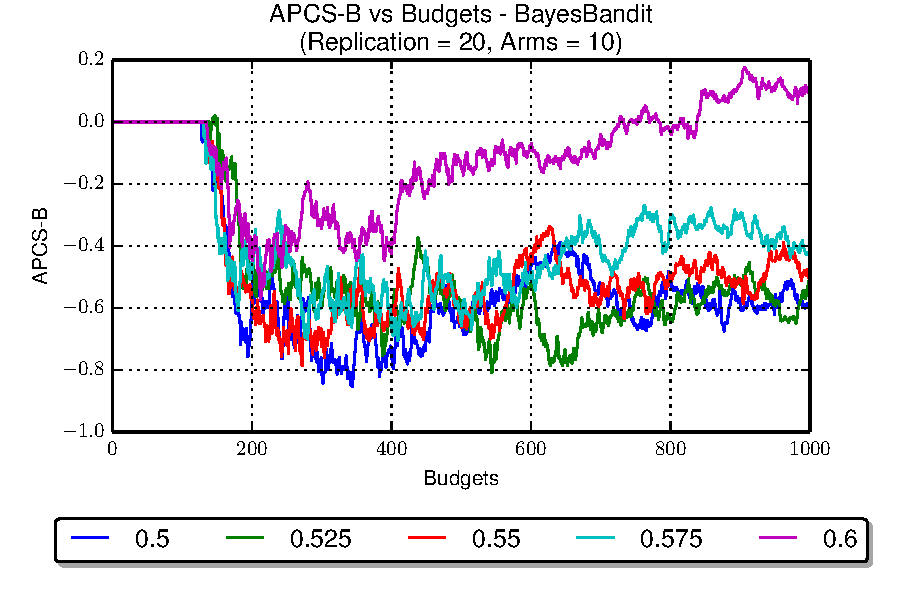
\includegraphics[page=1,width=\textwidth]{7BayesBandit_rate_series_pcs.pdf}
\end{figure}
\begin{figure}[p]
    \centering
    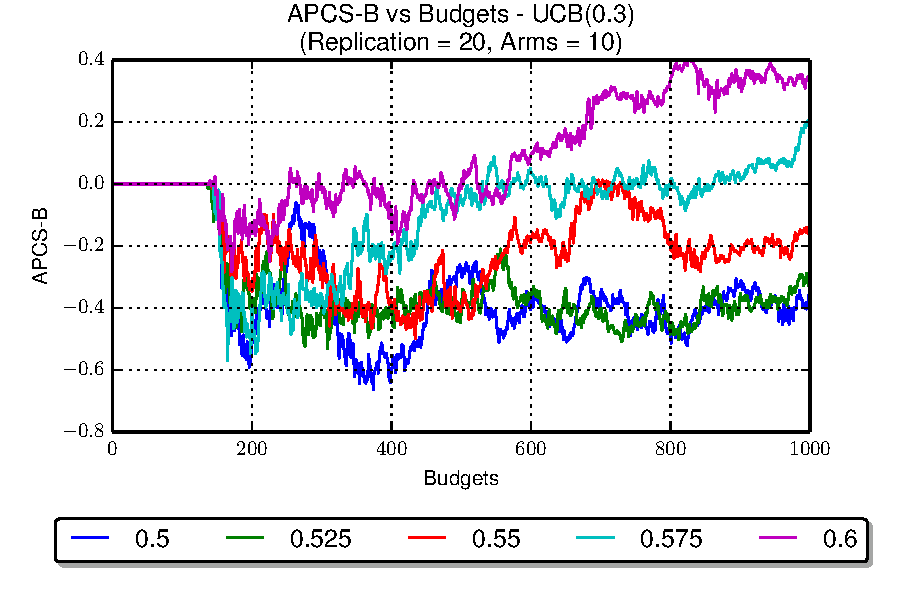
\includegraphics[page=1,width=\textwidth]{9UCB_rate_series_pcs.pdf}
\end{figure}
\end{minipage}%
\hfill
\begin{minipage}{0.48\textwidth}
\begin{tabular}{p{\textwidth}}
\begin{figure}[p]
    \centering
    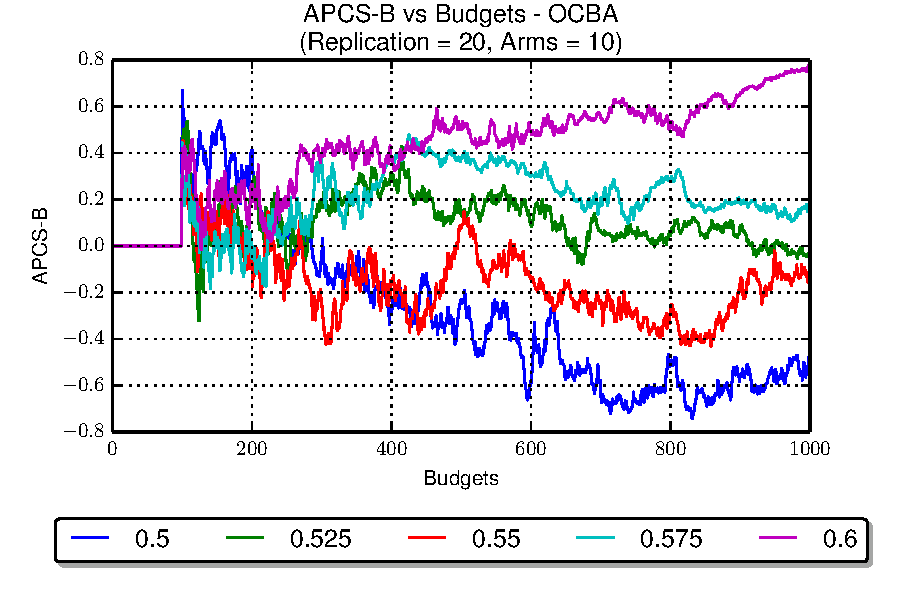
\includegraphics[page=1,width=\textwidth]{8OCBA_rate_series_pcs.pdf}
\end{figure}
\begin{itemize}
\item Not very useful for UCB and BayesBandit. \\
\item OCBA performance is a lot better.
\end{itemize}
\end{tabular}
\end{minipage}%
\end{frame}

\subsection{Change in Initial Budget (OCBA)}

\begin{frame}
\smaller
\begin{minipage}{0.48\textwidth}
\begin{figure}[p]
    \centering
    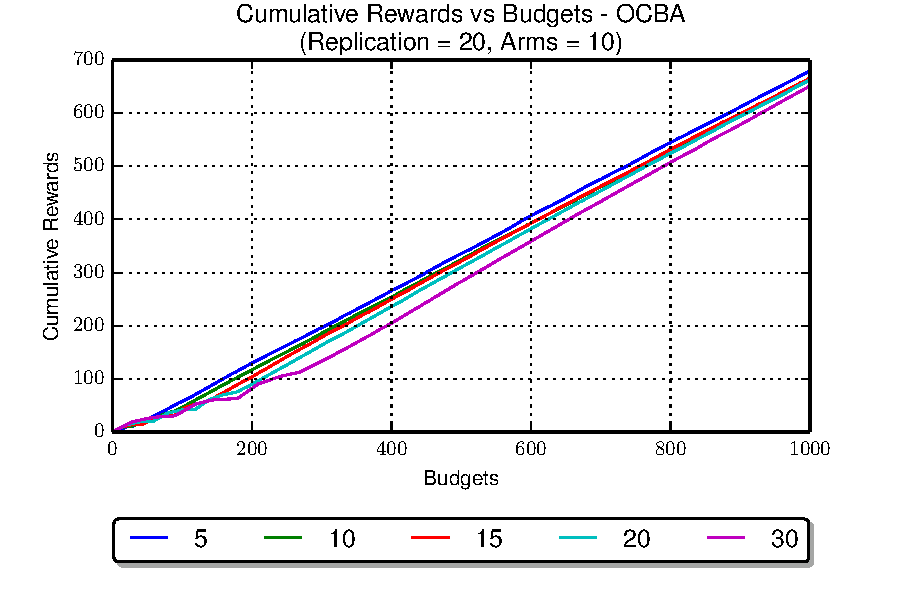
\includegraphics[page=1,width=\textwidth]{4OCBA_initsim_series_cumulative_rewards.pdf}
\end{figure}
\begin{figure}[p]
    \centering
    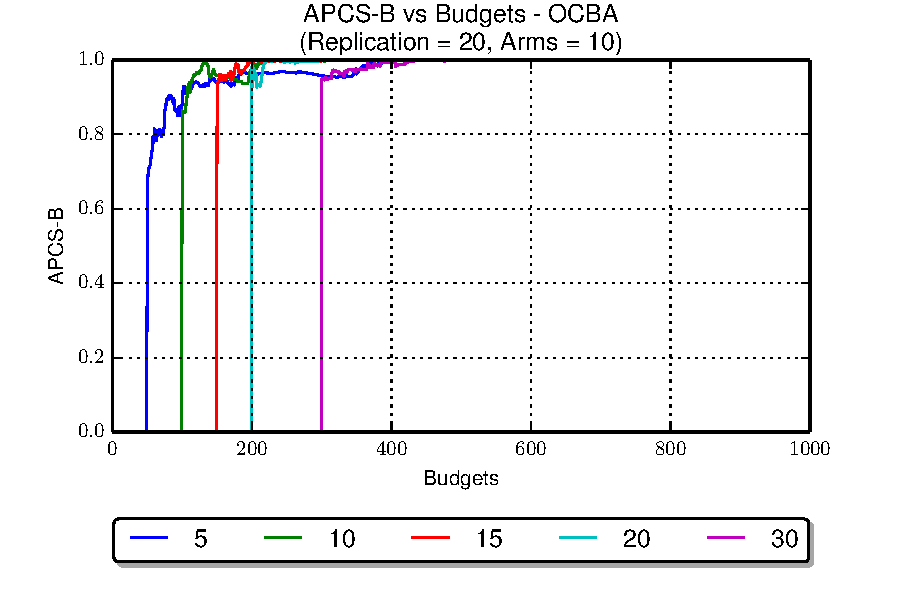
\includegraphics[page=1,width=\textwidth]{10OCBA_initsim_series_pcs.pdf}
\end{figure}
\end{minipage}%
\hfill
\begin{minipage}{0.48\textwidth}
\begin{tabular}{p{\textwidth}}

\begin{itemize}
\item Regardless of the initial budget allocation, the different experiments converge. \\
\item The convergence towards a APCS-B of 1 increases as the initial budget increases, saturating at around an initial budget of 15.
\end{itemize}
\end{tabular}
\end{minipage}%
\end{frame}

\subsection{Change in Budget}

\begin{frame}
\begin{figure}[p]
    \centering
    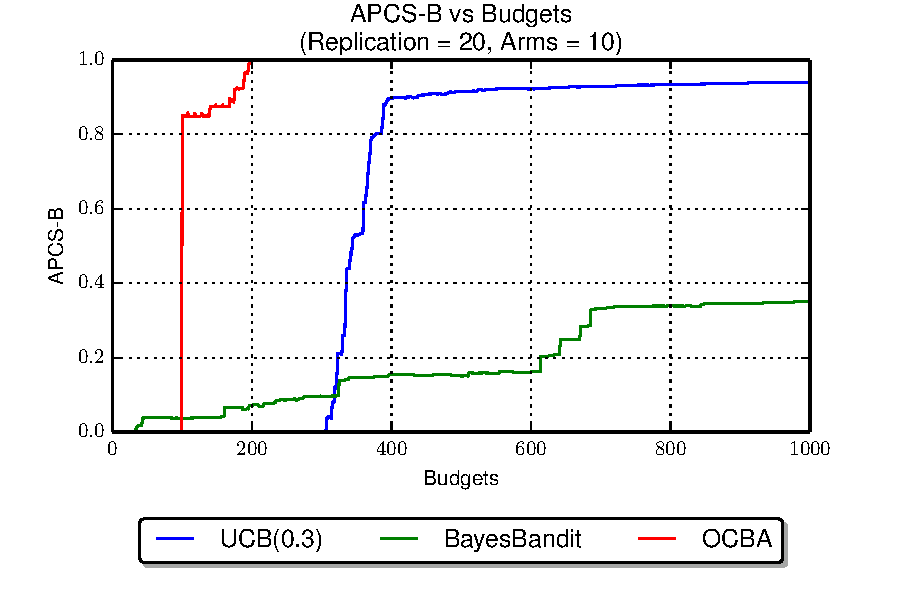
\includegraphics[page=1,width=0.8\textwidth]{11series_pcs.pdf}
\end{figure}
\begin{itemize}
\item UCB and OCBA show promising convergence\\
\item OCBA is faster at obtaining the desired result
\end{itemize}
\end{frame}


\begin{frame}
\smaller
\begin{minipage}{0.48\textwidth}
\begin{figure}[p]
    \centering
    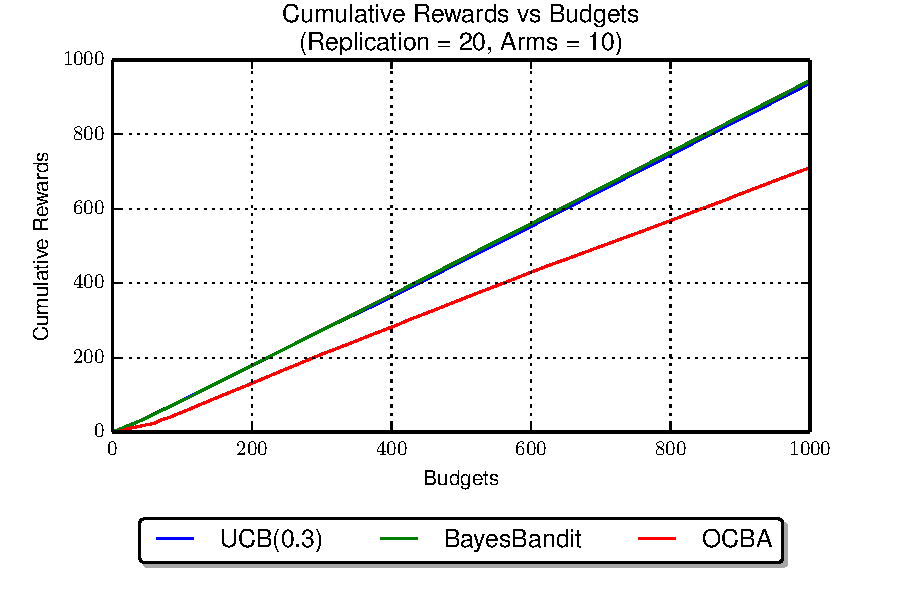
\includegraphics[page=1,width=\textwidth]{5series_cumulative_rewards.pdf}
\end{figure}
\begin{figure}[p]
    \centering
    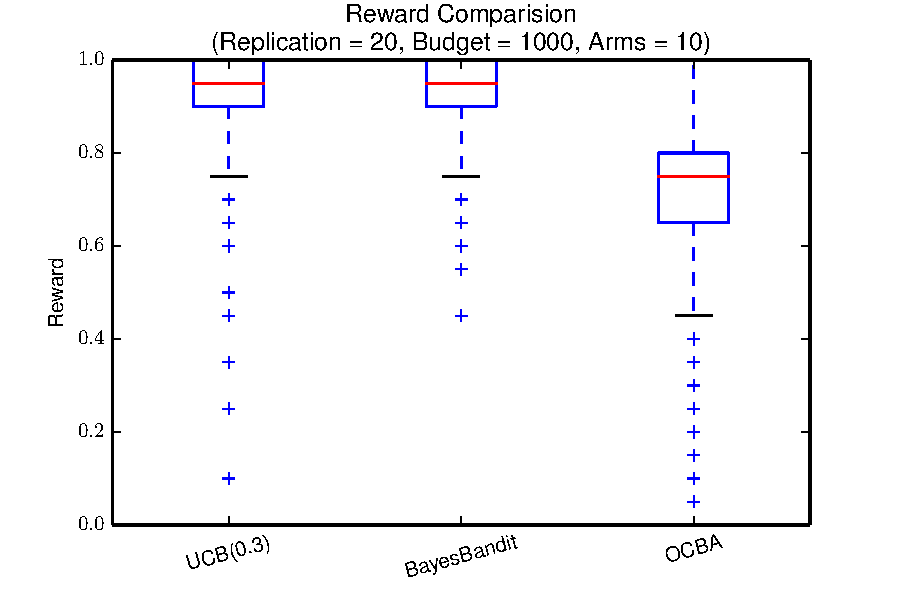
\includegraphics[page=1,width=0.8\textwidth]{6boxplot_rewards.pdf}
\end{figure}
\end{minipage}%
\hfill
\begin{minipage}{0.48\textwidth}
\begin{tabular}{p{\textwidth}}
\begin{itemize}
\item The performance of UCB and BayesBandit are largely superior to that of OCBA. \\
\item This shows that the focus of OCBA is not on obtaining the highest profit.
\end{itemize}
\end{tabular}
\end{minipage}%
\end{frame}



\subsection{Comparison of Efficiency}
\begin{frame}
\begin{figure}[p]
    \centering
    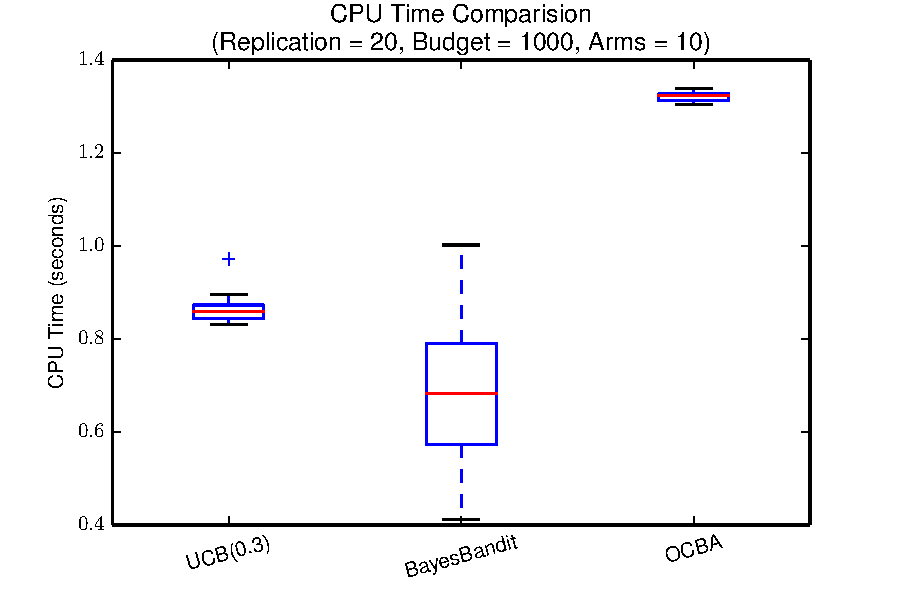
\includegraphics[page=1,width=0.8\textwidth]{12boxplot_cpu_time.pdf}
\end{figure}
\begin{itemize}
\item Though OCBA seems to be more complex, the difference is still counted as negligible for simple experiments. This difference may be more significant when dealing with more complicated rewards distributions.
\end{itemize}
\end{frame}

\section{Conclusion}

\subsection{}

\begin{frame}
Summary of the different Algorithms
\begin{itemize}
\item OCBA converges the fastest in terms of finding the Probability of Correct Selection, but UCB provides the largest reward in the long run. 
\item A suggestion is to perform the OCBA algorithm in the initial warm-up stages and switch over to the UCB after.
\item While the BayesBandit case shows an overall good performance, prior information about the distribution needs to be known, and its effectiveness may decrease if we use the wrong distribution.
\end{itemize}
\end{frame}

\begin{frame}
\Huge{\centerline{Thanks!}}
\centerline{Q\&A}
\end{frame}

\end{document} 
